
\section{Proposed Methodology}\label{sec:5_first_proposed_approach}

In this section, we present the primary phases of our study, which consist of three distinct steps designed to address the challenges of handling emerging new classes in drifted streams. Our proposed approach aims to develop a robust framework capable of tackling these complex challenges through a comprehensive, three-step methodology.
\begin{itemize}
	\item \textbf{Emerging New Classes:} Our study addresses the widespread issue of emerging new classes in drifted streams using well-known techniques, including concept drift detection and K-means clustering.
	\item \textbf{Drifted Streams: } To handle changes in the data distribution, our approach integrates a concept drift detector that dynamically identifies shifts, allowing the model to promptly adapt its classifiers to maintain effectiveness.
	\item \textbf{Classifier Performance:} The final phase identifies unknown classes in drifted streams, creating new classifiers for emerging classes to improve the model's ability to classify new instances accurately.
\end{itemize}

\subsection{THE PROPOSED APPROACH Flow}

Our proposed approach is designed with three distinct phases that work together to improve its performance in managing multiclass imbalanced and drifting data streams. 
\begin{itemize}
	\item \textbf{DES Phase (dynamic ensemble selection phase):} The first phase, known as the dynamic ensemble selection (DES) phase, is responsible for selecting the most appropriate classifier for the incoming data. This ensures that the selected classifier is well-suited for the current data chunk.
	\item \textbf{Drift detector phase:} The second phase of our approach is the drift detector phase, which operates in real-time to continuously monitor the data stream. Its primary function is to identify any signs of concept drift, which indicates shifts in the underlying data distribution over time.
	\item \textbf{Emerging New Class Identifier Phase:} The final phase of our approach is the synthetic data generator phase, which is dedicated to generating synthetic data for the minority classes. This step is crucial for addressing class imbalance by producing additional samples for underrepresented classes, thereby significantly enhancing the model's ability to accurately classify instances from minority classes.
\end{itemize}

As depicted in Fig. \ref{fig:5_first_proposal_step_1}, the DES phase retrieves the current data chunk and applies the DES technique to select the best classifiers for the chunk (black box of Fig.  \ref{fig:5_first_proposal_step_1}). These classifiers are used in the second phase to predict class labels, while drift detectors like ADWIN or DDM monitor for concept drift. If a drift is detected (highlighted by the red rectangle), the chunk is forwarded to the third phase, where new classes are identified (see Fig.  \ref{fig:5_first_proposal_step_2}). The overall approach is implemented in Algorithm  \ref{alg:5_1}, which takes a data stream and a DES Pool threshold as inputs. Key components include training the initial ensemble (Lines 4-6), using DES to select the best classifier for the current chunk (Line 8), detecting drifted chunks (Line 10), creating new classifiers for emerging classes (Line 12), and removing the worst classifier if the DES Pool threshold is exceeded (Lines 14-16).


\subsection{Emerging New Classes Phase Details}

In this section we present the Emerging new classes phase details. As shown in Fig.2, The emerging phase contains two primary steps: 
\begin{itemize}
	\item 	\textbf{Emerging new classes identifier:} The emerging class detection step plays a crucial role in the proposed approach (the black rectangle of Fiq.2) by utilize the K-means technique to clustering the drifted chunk into a set of clusters. And identifying new emerging classes by evaluating the distances between instances and their nearest class centroid. This process involves comparing the distance between an instance and the nearest class centroid with the maximum distance between class centroids ($d_c$), as described in Eq. \ref{eq:5_first_proposal_1} and Eq. \ref{eq:5_first_proposal_2}, where ED represents the Euclidean Distance method and ci, cj denotes the centroids of the current classes. If the calculated distance ($d_x$) exceeds this threshold ($d_c$), this indicates the presence of a new emerging class, denoted by EC in Eq. \ref{eq:5_first_proposal_3}; otherwise, it is $P_\text{DES}$ (prediction class of the new instance).
	\item \textbf{Adaptive the Emerging classes pool size:} This critical step adapts the pool size based on the emergence rate of new classes and drift distribution, using statistical measures like standard deviation, first derivative, and average historical drift updates.
	The Emerging New Classes phase is implemented in Algorithm  \ref{alg:5_2}, which utilizes drifted instances and current changes as inputs. Key steps include applying K-means (Line 1), calculating cosine similarity between centroids (Line 2), determining the maximum centroid distance (Line 3), setting the adaptive pool threshold (Lines 4-7), using KNN to find the nearest neighbor (Line 9), storing instances in the emerging pool if the distance exceeds the threshold (Lines 11-12), and creating a new classifier if the pool size surpasses the adaptive limit (Lines 14-17). A simulated scenario is illustrated in Figures 3 and 4. In Fig. \ref{fig:5_scenario1}(a), the drifted chunk is divided into three clusters using the K-means algorithm. Fig. \ref{fig:5_scenario1}(b) shows the calculation of the maximum distance between cluster centroids, which serves as a threshold for identifying new classes. The procedure for classifying instances is as follows: when a drifted instance is detected, it is considered a new class if the distance between the instance and its nearest centroid exceeds the maximum inter-centroid distance (Fig. \ref{fig:5_scenario2} a). If the distance is within the threshold, the instance is classified as a known class (Fig. \ref{fig:5_scenario2} b).
\end{itemize}

\begin{figure}[!ht]
	\centering
	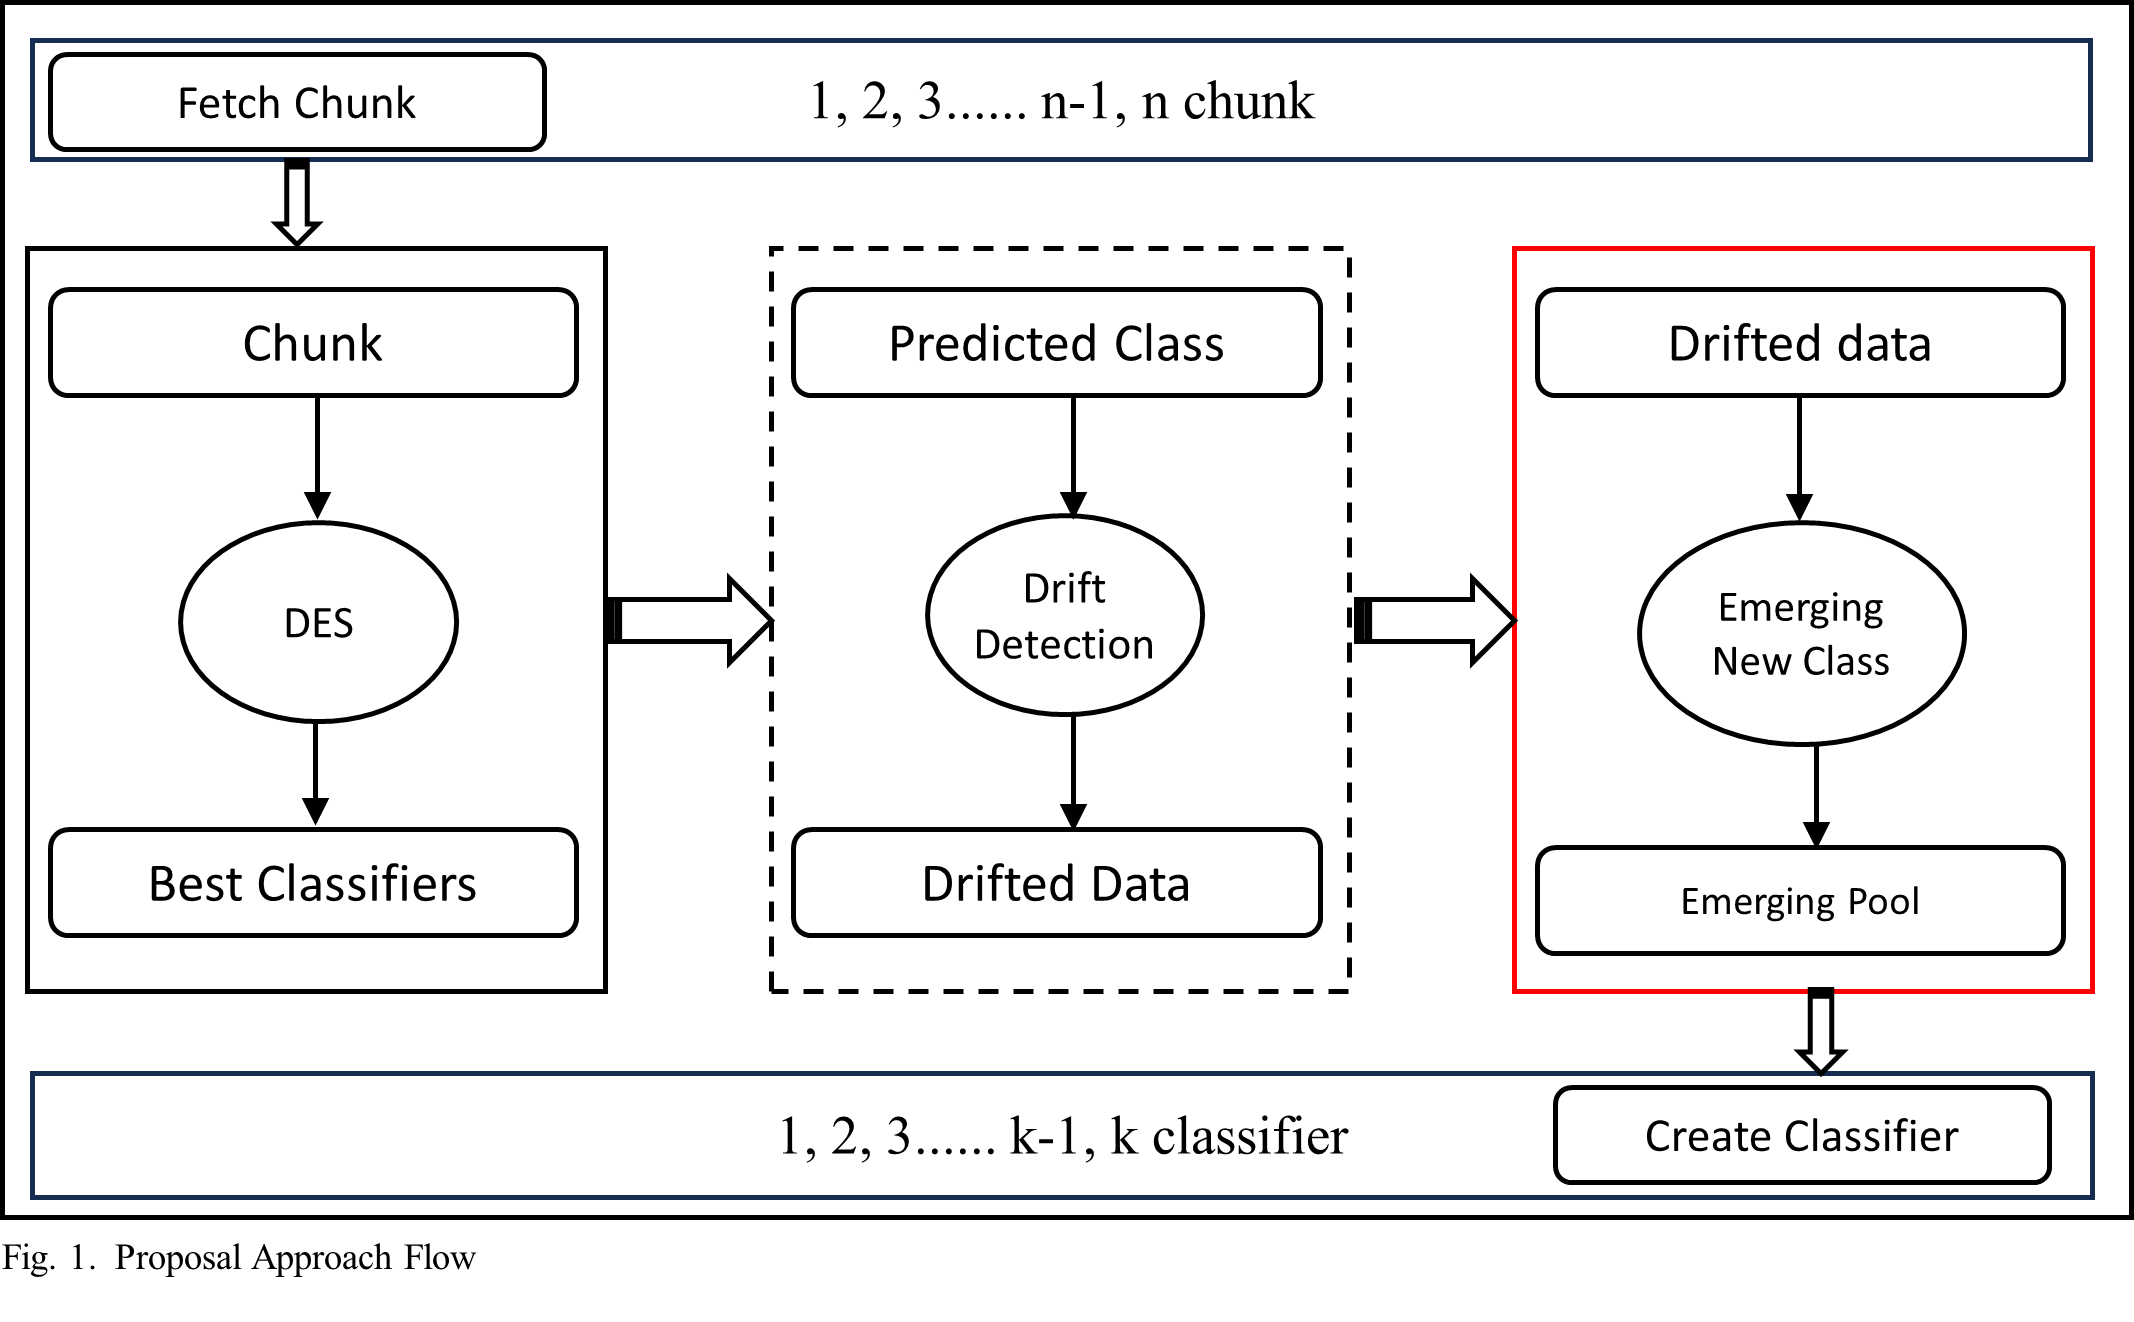
\includegraphics[width=1\linewidth]{5_Emerging/figures/algorithm1.png}
	\caption{Proposed Approch Flow}
	\label{fig:5_first_proposal_step_1}
\end{figure}
\begin{figure}[!ht]
	\centering
	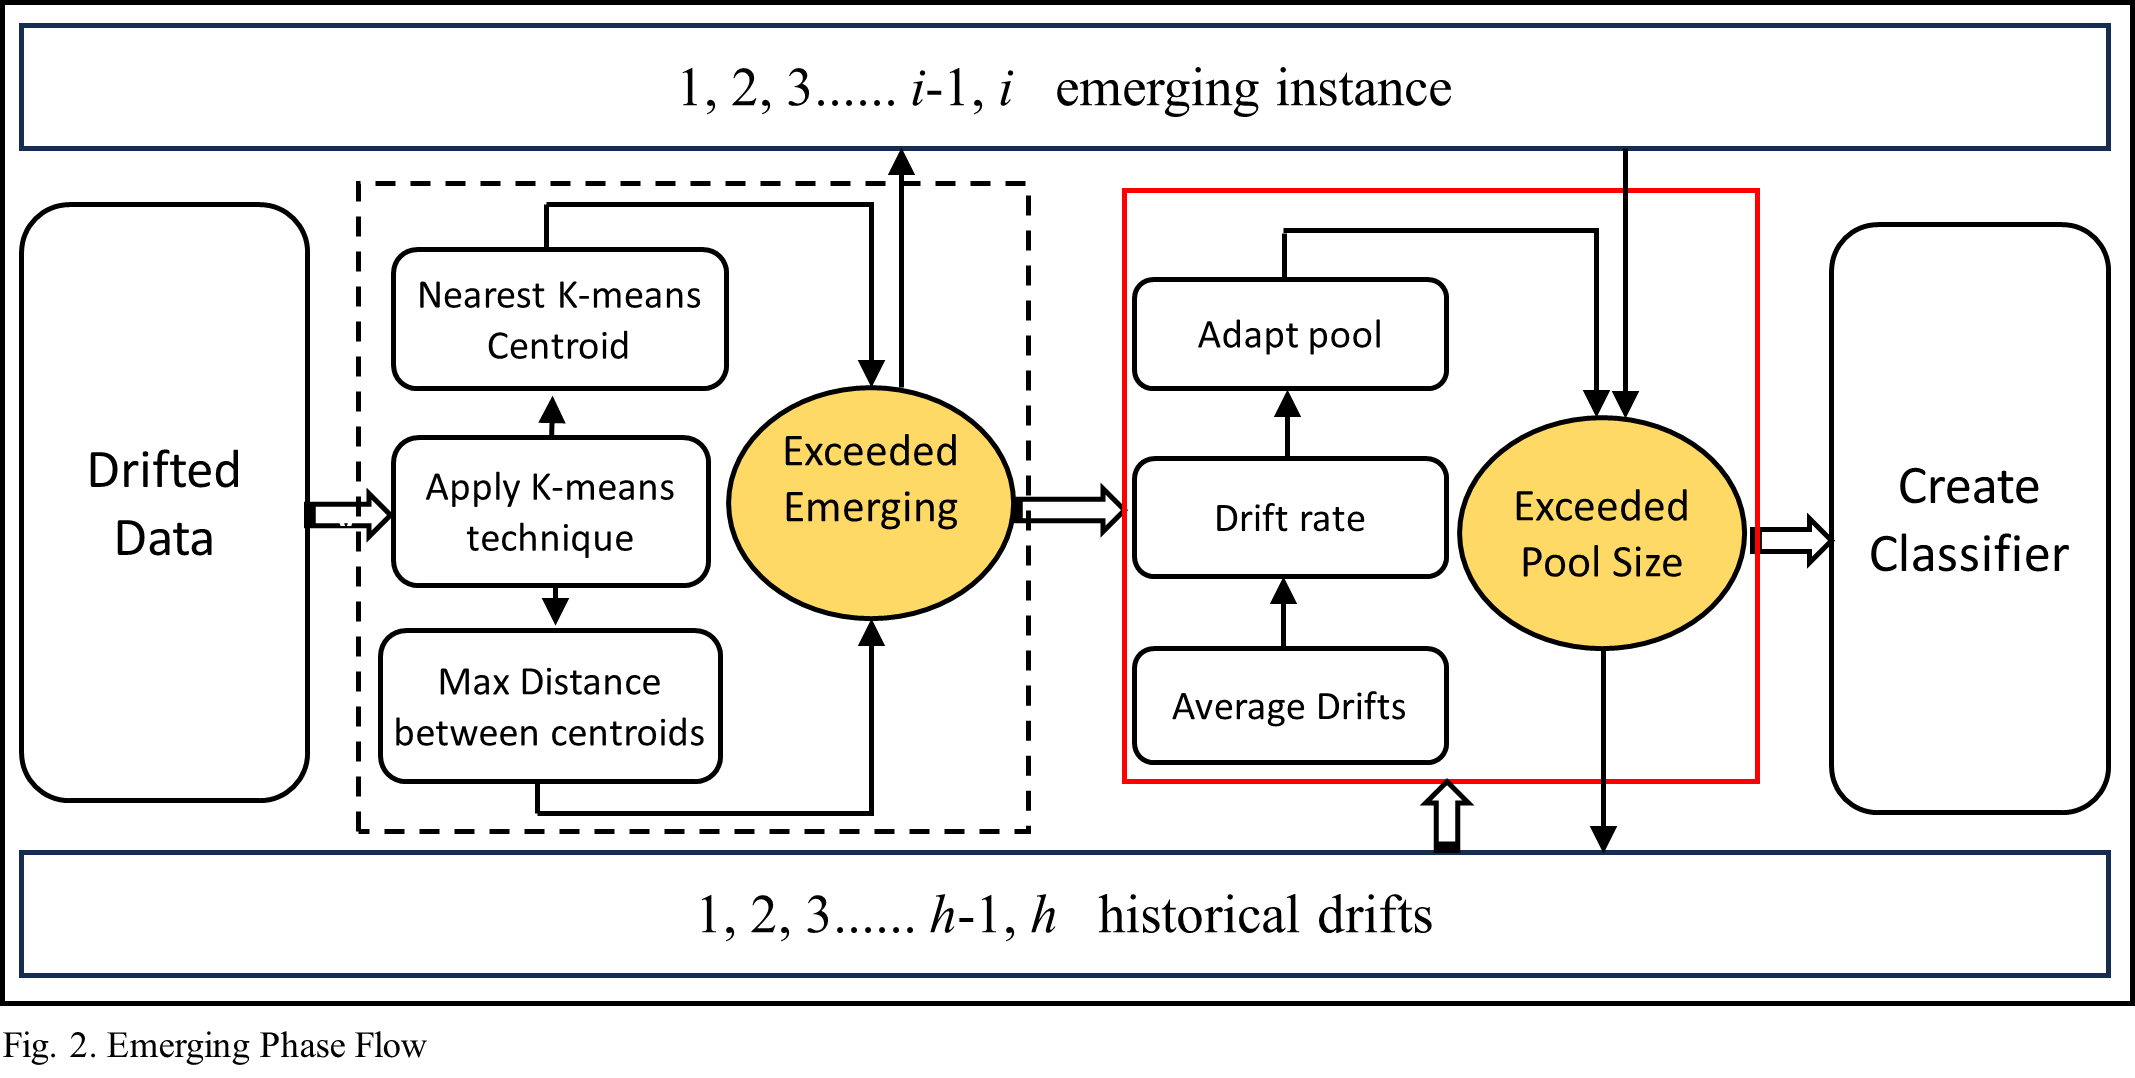
\includegraphics[width=1\linewidth]{5_Emerging/figures/algorithm2.png}
	\caption{Emerging Phase Flow}
	\label{fig:5_first_proposal_step_2}
\end{figure}
\begin{figure}[!ht]
	\begin{center}
	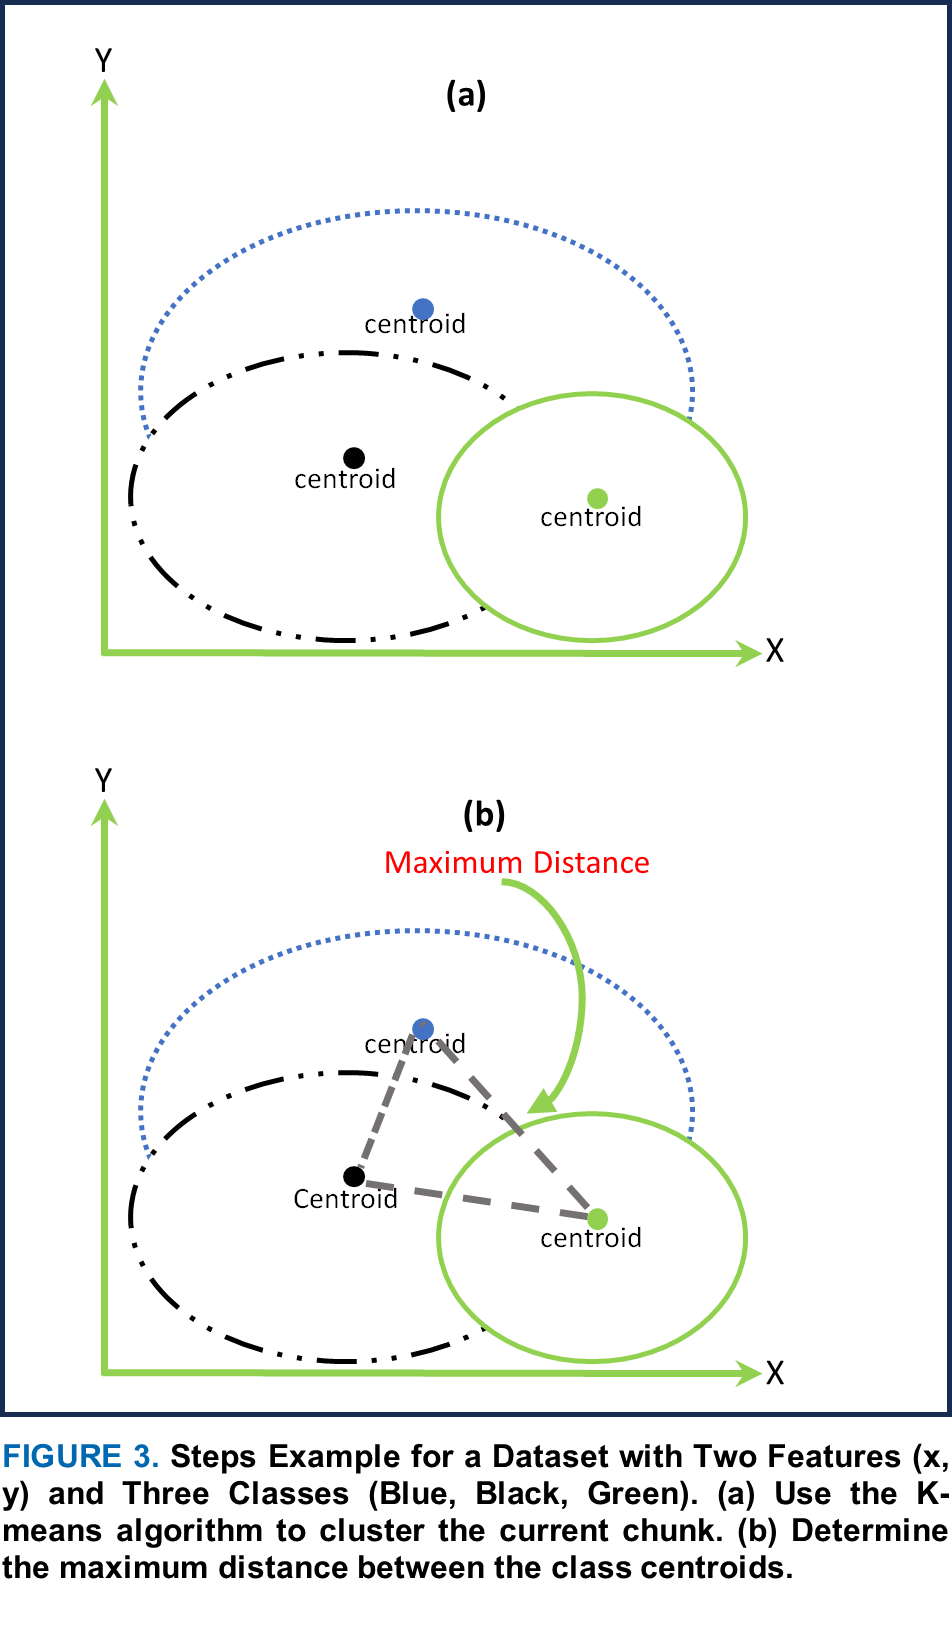
\includegraphics[width=0.48\linewidth]{5_Emerging/figures/scenario1.png}
	\caption{Proposed Approch Flow}
	\label{fig:5_scenario1}
	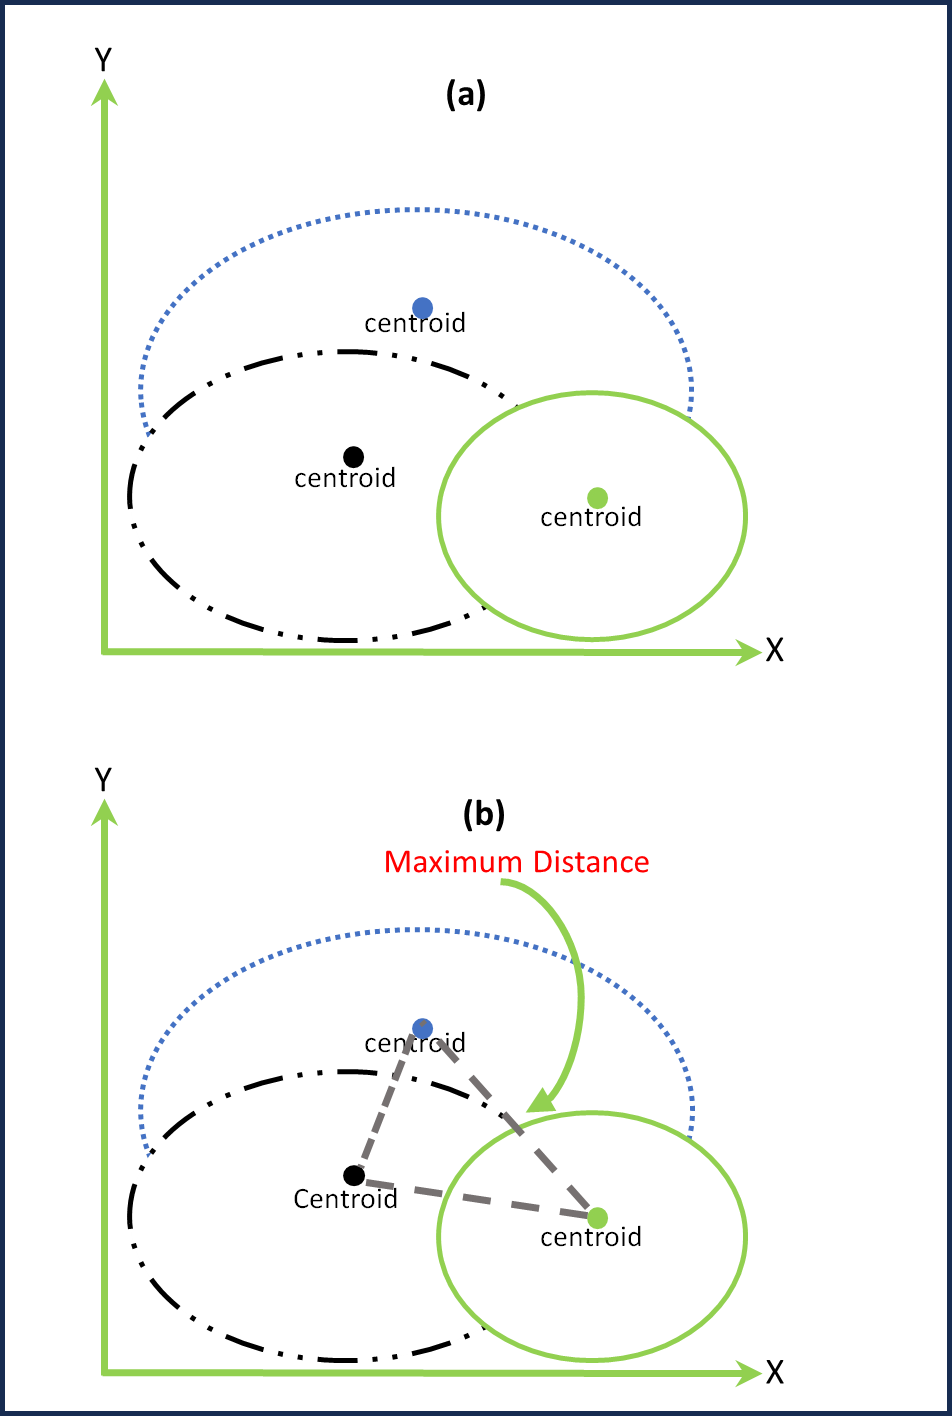
\includegraphics[width=0.48\linewidth]{5_Emerging/figures/senario2.png}
	\caption{Emerging Phase Flow}
	\label{fig:5_scenario2}
\end{center}

\end{figure}

\begin{equation}
	\label{eq:5_first_proposal_1}
    d_c = \arg\max_d \sum_{i=1}^{i} \sum_{j=i+1}^{i} d = ED(c_i, c_j)
\end{equation}

\begin{equation}
	\label{eq:5_first_proposal_2}
	d_x = \arg\min_i \sum_{i=1}^{i} ED(x, c_i)
\end{equation}

\begin{equation}
	\label{eq:5_first_proposal_3}
    \begin{cases}
		EC & \text{if } d_x > d_c \\
		P_{DES} & \text{otherwise}
	\end{cases}
\end{equation}

\begin{algorithm}[H]
	\caption{Proposed Framework Algorithm for Imbalanced Multi-Class Drifted Data Streams}
	\label{alg:5_1}
	\KwIn{data stream, maximum classifiers pool size $\kappa$}
	% \Parameter{current chunk $a$, synthetic data $b$, classifiers pool $\Psi$, drifted pool $\psi$, classes frequency $\Omega$, best frequency $\omega$, minority classes $\mu$}
	\KwOut{Prediction $P$}
	\BlankLine
	$\psi, \Psi, \Omega, \mu \gets \emptyset$\;
	$\omega \gets 0$\;
	\For{stream have chunk}{
		\eIf{$a$ is the First chunk}{
			$k \gets$ \texttt{trainingNewClassifier}($a$)\;
			$P \gets$ \texttt{getPrediction}($a, k$)\;
		}{
			$k \gets$ \texttt{DES}($a, \Psi$)\;
			$P \gets$ \texttt{getPrediction}($a, k$)\;
			$\psi \gets$ \texttt{conceptDriftDetector}($P$)\;
			\If{$\psi > 0$}{
				$\Omega \gets$ get classes frequency according to Eq.1\;
				$\omega \gets$ best frequency according to Eq.2\;
				$\mu \gets$ get minority classes according to Eq.3\;
				$b \gets$ utilize $a$ and $\mu$ to get the synthetic data according to Algorithm 2\;
				trainingData $\gets a + b$\;
				$k \gets$ \texttt{trainingNewClassifier}(trainingData)\;
				$\Psi \gets \Psi + k$\;
				\If{$\Psi > \kappa$}{
					\texttt{removeWorstClassifier}($\Omega$)\;
				}
			}
			$P \gets$ \texttt{getPrediction}($a, k$)\;
		}
	}
	\Return{$P$}
	\end{algorithm}
	
	\vspace{1cm}
	
	\begin{algorithm}[H]
		\caption{Synthetic data generator}
		\label{alg:5_2}
		\KwIn{Minority classes $\mu$, current chunk $a$, sample size $\eta$, historical chunks $h$}
		\KwOut{Generated data $b$}
		$b \gets \emptyset$\;
		$f \gets \text{MLSMSOTE}$\;
		$knn \gets \text{kNearestNeighbor}(a)$\;
		$chunk \gets \text{similarChunk}(a, h)$\;
		$f \gets \text{similarChunkOverSamplingMethod}(chunk)$\;
		\If{$f = \text{MLSMSOTE}$}{
			$f \gets \text{MLSOL}$\;
		}
		\Else{
			$f \gets \text{MLSMSOTE}$\;
		}
		\While{$|b| < \eta$}{
			$p \gets \text{generateSyntheticPoint}(\mu, f)$\;
			$similarPointsClass \gets \text{KNN.getKneighbor}(b)$\;
			\If{$similarPointsClass = \mu$}{
				$b \gets b \cup \{p\}$\;
			}
		}
		\Return $b$\;
		\end{algorithm}